\documentclass[11pt, a4paper, titlepage]{article}
\usepackage[left=2cm, right=2cm, top=2cm, bottom=2cm]{geometry}
\usepackage[style=authoryear,backend=bibtex]{biblatex}
\usepackage{helvet}
\renewcommand{\familydefault}{\sfdefault}
\usepackage{graphicx}
\linespread{1.25}
\usepackage[T1]{fontenc}
\usepackage{lineno}
\bibliography{Proposal}

\begin{document}

\linenumbers
\begin{titlepage} % Suppresses headers and footers on the title page
	
	\centering % Centre everything on the title page
	
	\scshape % Use small caps for all text on the title page
	
	\vspace*{\baselineskip} % White space at the top of the page
	
	%------------------------------------------------
	
	%	Title
	
	%------------------------------------------------
	
	\rule{\textwidth}{1.6pt}\vspace*{-\baselineskip}\vspace*{2pt} % Thick horizontal rule
	
	\rule{\textwidth}{0.4pt} % Thin horizontal rule
	
	\vspace{0.75\baselineskip} % Whitespace above the title
	
	{\LARGE Factors influencing the amphibian mycobiome, with a focus on known and unknown chytrids \\} % Title
	
	\vspace{0.75\baselineskip} % Whitespace below the title

	\rule{\textwidth}{0.4pt}\vspace*{-\baselineskip}\vspace{3.2pt} % Thin horizontal rule
	
	\rule{\textwidth}{1.6pt} % Thick horizontal rule
	
	\vspace{2\baselineskip} % Whitespace after the title block
	
	%------------------------------------------------
	
	%	Subtitle
	
	%------------------------------------------------
	
	MRes Project Proposal % Subtitle or further description
	
	\vspace*{3\baselineskip} % Whitespace under the subtitle
	
	%------------------------------------------------
	
	%	Editor(s)
	
	%------------------------------------------------
	
	\vspace{0.5\baselineskip} % Whitespace before the editors
	
	{\scshape\Large Supervisor:\\
		Prof Matthew Fisher \\
		Imperial College London\\} % Editor list
	
	\textit{matthew.fisher@imperial.ac.uk}

\end{titlepage}

%\title{Factors influencing amphibian mycobiome, with a focus on known and unknown chytrids}
%\author{Lucy Goodyear}
%\date{\parbox{\linewidth}{\centering%
%		\bigskip
%		Supervisor: Professor Matthew Fisher %\endgraf \bigskip
%		matthew.fisher@imperial.ac.uk \endgraf \bigskip
%		Dept.\ of Public Health \endgraf \bigskip
%		Imperial College}}


	%\maketitle

\noindent \textbf{Keywords}: Chytrid; Amphibian; Mycobiome; DNA barcoding; Fungus; Novel lineages

\section{Introduction and Proposed Questions}

\noindent Chytridiomycosis, caused by the amphibian chytrid fungus \textit{Batrachochytrium dendrobatidis} (\textit{Bd}), has been linked to a presumed 90 extinctions and the decline of over 500 more species in the past decades\parencite{Scheele2019}. Given the discovery of \textit{Batrachochytrium salamandrivorans} (\textit{Bsal}), a more recently emerged, highly virulent pathogen that is the sister taxon to \textit{Bd} \parencite{Martel2013}, and the prediction that more than 92\% of fungal species are yet to be described \parencite{hawksworth2017fungal}, it is likely that there are other undiscovered chytrids that parasitise amphibians. These are likely to be phylogeographically constrained endemic species that become tomorrow's emerging infections. Conversely, evolutionarily-distinct linages with superior competitiveness may provide protection against virulent strains, such as \textit{Bd} and \textit{Bsal}, through competitive exclusion \parencite{Hardin1960}. \newline

\noindent In the past few years, there has been an increase in research on the amphibian skin microbiome, for example that by \parencite{Bates2018} and \parencite{Bates2019} but little work specialising on the fungal communities present on amphibian skin, the mycobiome, and there has been no study on the factors influencing the diversity of the amphibian mycobiome globally. A global fungal composition analysis of the fungi that have evolved the ability to colonise, or even infect, amphibian skin would allow the association between different commensal fungi and \textit{Bd} and \textit{Bsal} to be determined for the first time. Negatively associated species may be evidence of niche exclusion \parencite{Hardin1960}, and positively associated species may represent secondary infections as a consequence of chytridiomycosis-associated dysbioses. This evidence could provide important groundwork for future conservation and novel promycotic treatments if strong negative associations are found.

\begin{list}{\labelitemi}{\leftmargin=1em}
	\item \textit{Which factors influence the amphibian mycobiome on a global scale?}
	
	\item \textit{What are the associations between \textit{Bd}, \textit{Bsal} and other fungal species in the amphibian mycobiome?}
	
	\item \textit{Are novel chytrid species a key link to providing a defence against virulent evolutionarily-distinct lineages or do they themselves pose a threat of becoming virulent in the future?} 
\end{list}

\section{Proposed Methods}

\noindent Over the past decade, amphibian skin swabs and environmental abiotic data have been collected for a variety of species and life stages from all over the world, allowing an analysis of the amphibian mycobiome to be done on a global scale for the first time. Using these processed data, it can be determined which commensal fungal species are present on large numbers of amphibian species from different populations and whether we can also detect unknown fungal species that may be pathogens. After accounting for potential autocorrelation and multiple comparisons, patterns can be identified and tested using statistical analyses in terms of possible influencing biogeographic factors, such as altitude, temperature, longitude and latitude etc. to deduce which factors better influence the composition of fungal species in an amphibian's mycobiome. These models will then be used to generate plots and GIS maps of locations of mycobiome similarity. The spread of \textit{Bd}, focusing on the novel lineages, will also be looked at using GIS. The R package \textit{cooccur} \parencite{RCooccur} will be used to analyse cooccurance between fungal species and \textit{Bd} to evaluate which fungi are positively and negatively associated with \textit{Bd}. Some of the unidentified fungal species could be unknown species of chytrid. Novel chytrid lineages will be identified through sequence alignment against pre-existing datasets in NCBI and by building phylogenetic trees in order to compare the candidate sequences with those of other chytrids. 

\section{Anticipated Outputs and Outcomes}

Statistically and biologically significant patterns in the mycobiome data will be determined in order to confidently predict which factors most influence the amphibian mycobiome. This will give an overview of the global amphibian mycobiome and help to understand why certain amphibians are affected by \textit{Bd} and \textit{Bsal}, both in terms of abiotic factors and in terms of the other fungal species that are present. Identification of previously unknown chytrid species that may act as promycotics, causing niche exclusion of a competing virulent species/lineage through prior occupancy, could contribute to pre-emptive conservation work against unknown virulent chytrids.

\section{Project Feasibility}

All data has already been collected using MiSeq 2x300bp v3 chemistry sequencing and almost all has already been processed and is ready for analysis. The time period for analysis and write up should be adequate to generate possible answers to all three of the above research questions. 

\begin{figure}[h!]
	\centering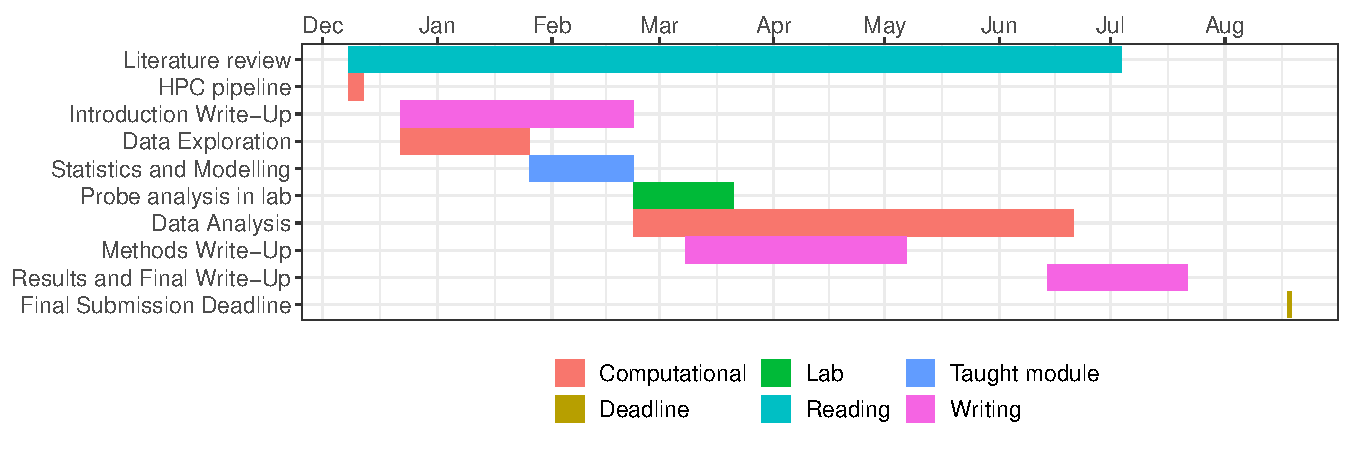
\includegraphics[width=1\textwidth]{GanttChart.pdf}
	\caption{Proposed Project Timeline}
\end{figure}

\begin{table}[h!]
	\small
	\begin{tabular} {| l | c | l |}  \hline
		\textbf{Budgeted Item} & \textbf{Cost} & \textbf{Reasoning} \\ \hline
		Herptofauna Workers Meeting 2020 & £250 & Herpetological conference cost and accommodation \\ \hline
		qPCR Reagents & £175 & To perform \textit{Bd} qPCR in the laboratory \\ \hline
		Laptop Adaptor & £75 & To enable me to use USB sticks, HDMI etc. with my laptop \\ \hline
		\textbf{Total} & £500  & - \\ \hline
	\end{tabular}
	\caption{Proposed Project Budget}
\end{table}

\newpage

\printbibliography

\newpage

\section{Approval}

I have seen and approved the proposal and the budget. 
\newline
\newline
\newline
\noindent Name:
\newline
\newline
\newline
\newline
Signature:
\newline
\newline
\newline
\newline
Date:

\end{document}
